\documentclass[a4paper, 12pt, openany]{book} %chose the paper size and font size. Openany ensures that all all chapters and similar may begin at any page, not only odd pages. For the introductory pages and appendices we want openany, but for chapter pages in the main content we want chapters to begin only on odd pages (right hand side). The book class ensures that the margins are automatically adjusted such that left hand pages are slightly moved to the left and vice versa at the right, which makes the thesis very readable and good looking when printed in bound book format.
\usepackage[utf8]{inputenc} %to manage special characters
\usepackage[T1]{fontenc} %to manage special characters
\usepackage[Bjarne]{fncychap} %fancy chapter style (many more available, like Sonny or Lenny etc.)
\usepackage{fancyhdr} %to customize the headers

\usepackage{multirow}
\renewcommand{\arraystretch}{1.2} % Adjust row height for better 

\usepackage[lmargin=1.5in, rmargin=1in, tmargin=1in, bmargin=1in]{geometry} %sets the margins for the pages
\setcounter{tocdepth}{2} %table of contents number depth for subsections (2 = x.x.x)
\setcounter{secnumdepth}{4} %numbering depth for headers for subsections in the text(4 = x.x.x.x)
\usepackage{url} %to include urls
\usepackage{listings} %include this if you want to include code in the thesis
\usepackage{amsmath,amssymb} %mathematical package
\usepackage{siunitx} %includes SI-units
\usepackage[bf]{caption} %makes float captions bold
\usepackage{array, booktabs} %to make better tables
\usepackage{graphicx} %to include graphics
\usepackage{float} %to include floats
\usepackage[export]{adjustbox} %to adjust floats
\usepackage{subfig} %to include subfigures
\usepackage{chngcntr} %will make it possible to change the counter for tables, figures etc. such as below
\counterwithin{figure}{section} %change counter for figures within sections (also possible to choose for each chapter
\counterwithin{table}{section} %change counter for tables within sections
\usepackage{color, xcolor} %edit e.g. text colors
\usepackage[pdftex]{hyperref} 			% Load hyperref as last to avoid compatibility issues
\hypersetup{  
	%bookmarks=false,    			% show bookmarks bar?
	unicode=true,      			% non-Latin characters in Acrobat’s bookmarks
	pdftoolbar=false,    			% show Acrobat’s toolbar?
	pdfmenubar=true,    			% show Acrobat’s menu?
	pdffitwindow=true,   			% window fit to page when opened
	pdfstartview={FitH},  			% fits the height of the page to the
	%pdfcreator={},  		% creator of the document
	%pdfproducer={}, 			% producer of the document
	pdfkeywords={master thesis, NTNU}, % list of keywords
	pdfnewwindow=true,   			% links in new window
	pdfdisplaydoctitle=true,  
	colorlinks=true,    			% false: boxed links, true: colored links
	linkcolor=black,     			% color of internal links
	citecolor=black,%NTNUBlue,    			% color of links to bibliography
	filecolor=black,%magenta,   			% color of file links
	urlcolor=black,%cyan,      			% color of external links
	bookmarksnumbered=true,
	bookmarksdepth=1%
}


\usepackage[backend = biber,
            style = numeric,
            date = long,     % Long: 24th Mar. 1997 | Short: 24/03/1997
            sorting = none,
            maxcitenames = 3,   % max names to include before et. al.
            ]{biblatex} %customize the look of your citations and bibliography
\addbibresource{bibliography.bib} %declare the bibliography resource
\usepackage{comment} %to be able to comment out sections in the .tex files
\usepackage{afterpage} %to customize page commands such as below
\newcommand\myemptypage{
    \null
    \thispagestyle{empty}
    \addtocounter{page}{-1}
    \newpage
    } %sets new page command to insert an empty page without adding to the page counter or having a page number

% \usepackage[none]{hyphenat}


\begin{document}
%%%%%%%%%%%%%%%%%%%%%%%%%%%%%%%%%%%%%%%%%%%%%%%%%%%%%%%%
%\begin{comment}
% The title page:
% For NTNU students this page will be generated automatically when submitting your paper, and should not be included in the final file from Latex. Delete or comment out the title page setup. The final report should then start with the first page being the abstract. I have included a title page here so it is possible to see how it may look like, and for those who does not get an automatically generated title page. Of course you will need to change the names and titles etc. to your case.

%the title page should be an odd page (right hand side)

\begin{titlepage}
\newgeometry{left=1.6in, right=2in}
\vspace*{1.5cm}

\noindent  \textcolor{gray}{\large Trygve Maukon Myhr} \\
\vspace{0.5cm}

\noindent \textbf{\Large Creating Synthetic Datasets for Revolt: Improving Autonomous Boat Docking with Computer Vision} \\
\vspace{0.5cm}

\noindent {\large Project Thesis} \\



\vspace{7cm}
\noindent Project Thesis in Robotics and Automation \\
Supervisor:\\
Co-supervisor: \\
December 2024\\

\vspace{0.2cm}
\noindent Norwegian University of Science and Technology \\
Faculty of Engineering \\
Department of Mechanical and Industrial Engineering \\

\begin{figure}[h]
    
\includegraphics[width=0.4\textwidth]{Figures/logo.png}
\end{figure}
\end{titlepage}
\restoregeometry
\myemptypage %empty page such that the abstract starts at the first right hand side after the title page
%\end{comment}
%%%%%%%%%%%%%%%%%%%%%%%%%%%%%%%%%%%%%%%%%%%%%%%%%%%%%%%%

% The pre-chapters
\chapter*{Abstract} %pre-chapters should not be numbered, hence the "*"
\pagenumbering{roman} %introductory pages should be roman
\setcounter{page}{1}
\addcontentsline{toc}{chapter}{\protect\numberline{}Abstract} %add the chapter to the table of contents, this is not automatically added when creating unnumbered chapters (*). Add it in a chapter style, and keep all chapters on the same numberline indent regardless of number or not on the chapter

This thesis explores the creation of synthetic datasets for computer vision applications in maritime environments, with a focus on harbor scenarios for autonomous vessels. A key challenge in this field is the limited availability of diverse and high-quality real-world data for training computer vision models. Collecting data in maritime environments is often expensive and time-consuming, requiring specialized equipment and manual annotation. To address these challenges, synthetic datasets can be an alternative. Using Unity’s Perception package, along with custom randomizers, a synthetic dataset of 2,350 labeled images was created. The dataset includes common maritime objects such as boats, kayaks and buoys, and covers a broad range of varied environmental conditions, including changes in weather, lighting and camera angles.\\

\noindent The project demonstrates several benefits of synthetic data, including reduced costs, increased scalability and the ability to generate large datasets. It also addresses the challenges associated with the domain gap between synthetic and real-world data. By implementing techniques such as AI-driven enhancements and randomization, the realism and diversity of the dataset are improved, making it more suitable for real-world applications, such as autonomous vessels in harbor environments.
 %insert the chapter text from the files

\chapter*{Preface}
\addcontentsline{toc}{chapter}{\protect\numberline{}Preface} 

Write the preface of your thesis here. \\

\noindent You may include acknowledgements and thanks as part of your preface on this page, or you may add it as a new chapter after the preface.

\tableofcontents
\addcontentsline{toc}{chapter}{\protect\numberline{}Contents}

%add to table of contents list of figures and tables, and insert list of figures and tables
\addcontentsline{toc}{chapter}{\protect\numberline{}\listfigurename}
\listoffigures
\addcontentsline{toc}{chapter}{\protect\numberline{}\listtablename}
\listoftables


\chapter*{Abbreviations}
\addcontentsline{toc}{chapter}{\protect\numberline{}Abbreviations}
% Put in your abbreviations here

List of all abbreviations in alphabetic order:

\begin{itemize}

    \item \textbf{2D}: Two-dimensional
    \item \textbf{3D}: Three-dimensional
    \item \textbf{3DS}: 3D Studio (file format)
    \item \textbf{AI}: Artificial Intelligence
    \item \textbf{C\#}: A programming language
    \item \textbf{CV}: Computer Vision
    \item \textbf{CVAT}: Computer Vision Annotation Tool
    \item \textbf{DAE}: Digital Asset Exchange (file format)
    \item \textbf{DNV}: Det Norske Veritas
    \item \textbf{DXF}: Drawing Exchange Format
    \item \textbf{FBX}: Filmbox (file format)
    \item \textbf{GANs}: Generative Adversarial Networks
    \item \textbf{ML}: Machine Learning
    \item \textbf{NTNU}: Norwegian University of Science and Technology
    \item \textbf{OBJ}: Object (file format)
     \item \textbf{R-CNN}: Region-based Convolutional Neural Network
    \item \textbf{RGB}: Red, Green, Blue
    \item \textbf{RGBA}: Red, Green, Blue, Alpha
    \item \textbf{ROS2}: Robot Operating System 2
    \item \textbf{UML}: Unified Modeling Language
    \item \textbf{UiT}: University of Tromsø – The Arctic University of Norway
\end{itemize}
    
    
\newpage
\myemptypage
%add an empty non-counted page by the command below in order to get the first chapter on the left hand side, if needed (check your page number so that the first chapter is on an odd page)


%%%%%%%%%%%%%%%%%%%%%%%%%%%%%%%%%%%%%%%%%%%%%%%%%%%%%%%%
%Customize the layout of the main content of your thesis

\pagestyle{fancy} %set customized page style for header
\fancyhf{} %clear header and footer fields
\renewcommand{\headrulewidth}{0pt} %set to no rule
\fancyhead[LE, RO]{\thepage} %set the page number at left for even, right for odd pages
\fancyhead[RE, LO]{\leftmark} %set the chapter name at right for even, left for odd pages
%is is possible to design the header with the chapter as you wish, e.q. only the chapter or only the name, all lowercase instead etc.
%you could also design the footer if you wish, for example:
%\fancyfoot[LE, RO]{\thepage}
\setlength{\headheight}{14.49998pt} %set the header height


%%%%%%%%%%%%%%%%%%%%%%%%%%%%%%%%%%%%%%%%%%%%%%%%%%%%%%%%
%main content 

\pagenumbering{arabic}
\chapter{Introduction}

% The subsections written are only suggestions, to display how sections and subsections may look for your thesis


\section{Motivation}



\section{Project Description}


Is synthetic data sufficient to train a computer vision system for accurate boat docking, or is real-world data necessary to achieve optimal performance?

Can AI tools help close the domain gap between synthetic and real-world data?

\section{Structure of the Report}

\cleardoublepage

\chapter{Literature Study}

\section{Motivation}


\section{object detection}

\section{ntnu ferry}

\section{all struggle with image generation}
\cleardoublepage

\chapter{Theory: Synthetic Images}
% theroy syntethic images
Synthetic images are computer-generated images that simulate real-world scenes or objects. They are increasingly used in computer vision when collecting real-world data is either difficult, expensive or raises privacy concerns. These images are especially useful for training machine learning models for tasks like object detection and image classification. When generating synthetic data, developers can create datasets that meet specific needs, which is important for industries like healthcare, self-driving cars and near-shore ocean environment, where real-world data may be hard to gather \cite{jimaging8110310, safety}.

\section{Advantages of Synthetic Data for CV Models}

Deep learning models need a lot of data to work well and as they evolve, the need for large datasets keeps growing \cite{10.1145/3042064, nikolenko2021synthetic}. Synthetic data can help meet this demand and provide a solution with several advantages.
 
\subsection{Customization}
One of the key benefits of synthetic data is customization. Synthetic images allow developers to create and change environments to meet specific needs. A scene can include various objects, environments and camera setups. All of these can be adjusted to match the requirements of a particular application. Synthetic image generation can construct diverse and complex scenes, and recreate scenarios that would be difficult to capture in the real-world. The dataset can then contain the exact conditions and variations needed to train a model effectively \cite{jimaging8110310, rajpura2017objectdetectionusingdeep}.

\subsection{Ethics}
Another big benefit is ethics. Synthetic data solves privacy problems because it does not use real information. For example, in face recognition tasks, using synthetic faces eliminates the need to collect photos of real people, avoiding privacy concerns and consent issues. Similarly, in medical applications, synthetic data can replace real patient data, protecting privacy while still providing useful training material for AI systems \cite{jimaging8110310}.

\subsection{Randomization}
Randomization in synthetic data means adding variety to the dataset. It is important for creating a robust dataset, as it ensures the model is trained on diverse scenarios rather than a single repetitive situation \cite{borkman2021unityperceptiongeneratesynthetic}. A dataset full of similar images of the same scene will not help a model generalize well and may lead to overfitting. Overfitting occurs when a model performs well on training data but struggles to generalize to new unseen data \cite{Ying_2019}. Randomization helps prevent this issue by introducing small, controlled variations in the data, making the model more adaptable and better equipped to handle real-world variability.\\

\noindent Compared to manually collecting real images, randomization allows for the creation of an almost unlimited variety of scenarios in a short amount of time. With real-world data, obtaining different perspectives or environmental conditions might require extensive setup or access to rare situations, making synthetic data more efficient and scalable \cite{borkman2021unityperceptiongeneratesynthetic}. \\

\noindent Synthetic data allows for various types of randomization. Objects in a scene can change through transformations like rotation, scaling or color. Additionally, the background and environment can be modified, including factors such as weather and scene layout. Randomization can also be applied to the camera settings, such as adjusting the position, tilt or angle, to generate a variety of perspectives \cite{borkman2021unityperceptiongeneratesynthetic}.\\

\noindent This flexibility allows for the automatic generation of unlimited, diverse training data without manually changing each scene. Randomization scripts make it easier and faster to create a wide range of scenarios, increasing the robustness of the computer vision model.\\

\noindent Further details on the implementation of randomization in synthetic data generation will be explained in \ref{section:Implementation of Randomizers in Unity} and \ref{section:Integrated Randomizers}.


\section{Image Labeling}
Image labeling is important in computer vision because it helps models understand what each part of the image represents. Without labeled images, a model wouldn’t know what is right or wrong and can not train correctly \cite{Labelling}.\\

\noindent Labeling involves creating another image or annotation that defines where the object is located in the original training image. It works like an answer, giving the model the correct outputs to learn in training. During training, the model is given both the images and their labels. The model compares its predictions with the labeled data and makes adjustments to improve its accuracy. Over time and iterations, the model learns how to identify and classify objects in new images based on the labeled examples \cite{Labelling}.


\subsection{Labeling Methods}

There are different ways to label objects in images, depending on the level of detail needed. Two common methods are bounding boxes and segmentation.\\

\noindent Bounding boxes, as shown in Figure~\ref{fig:image2}, use rectangular regions to indicate the locations of objects. This method is simple and effective for tasks requiring approximate localization but does not provide detailed information about shapes or boundaries.\\

\noindent Segmentation, illustrated in Figure~\ref{fig:image3}, assigns a label to each pixel in an image, distinguishing objects from their surroundings. This method offers detailed boundary information by dividing the image into regions, often represented with unique colors or patterns for different objects. Unlike bounding boxes, segmentation captures the exact shapes and fine details of objects, enabling a pixel-level understanding of the image \cite{labelingMethods}.\

\begin{figure}[H]
    \centering
    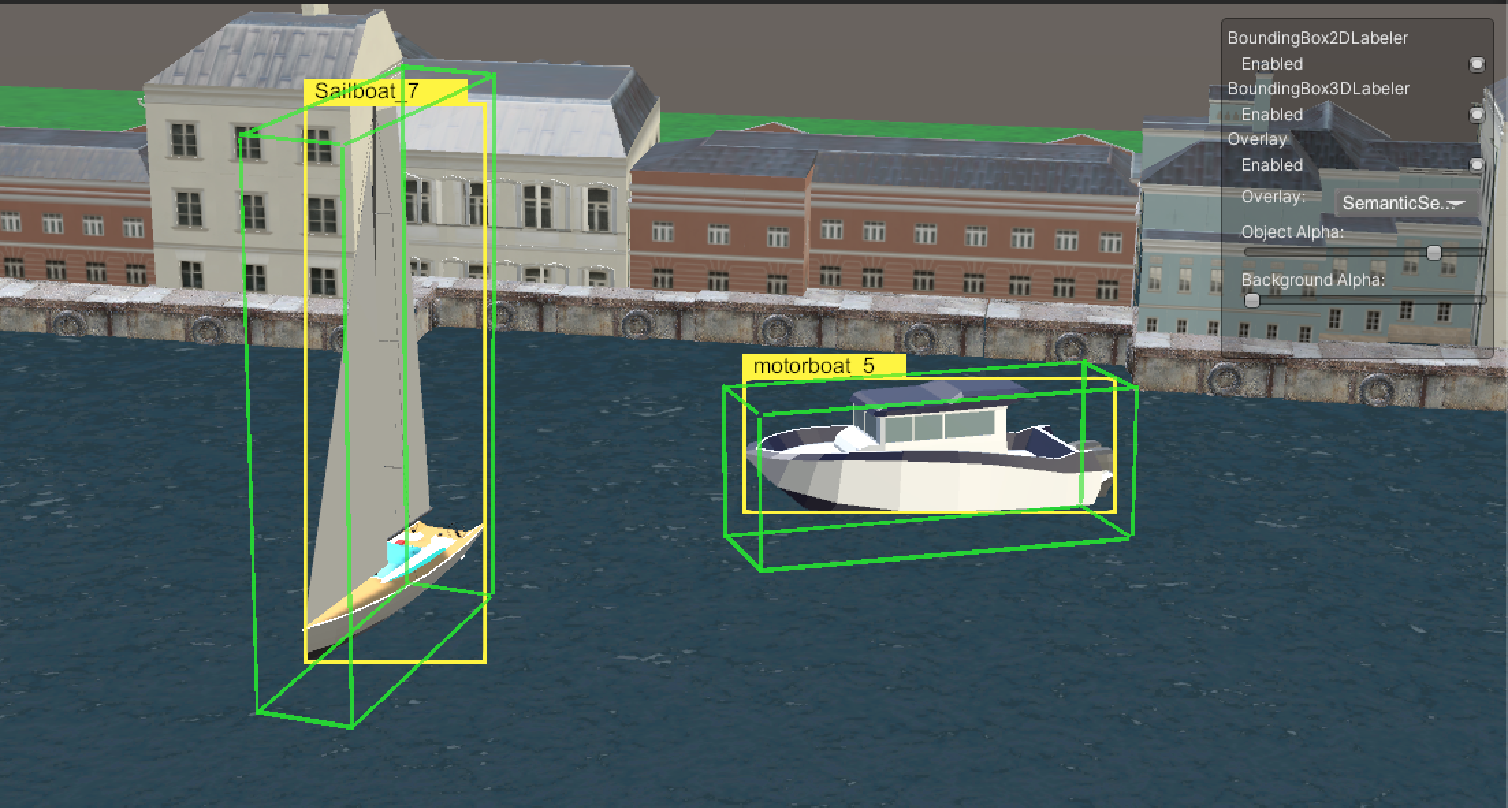
\includegraphics[width=0.7\textwidth]{Figures/boundingbox.png}
    \caption{Illustration of bounding boxes, with rectangular regions used to localize objects.}
    \label{fig:image2}
\end{figure}

\begin{figure}[H]
    \centering
    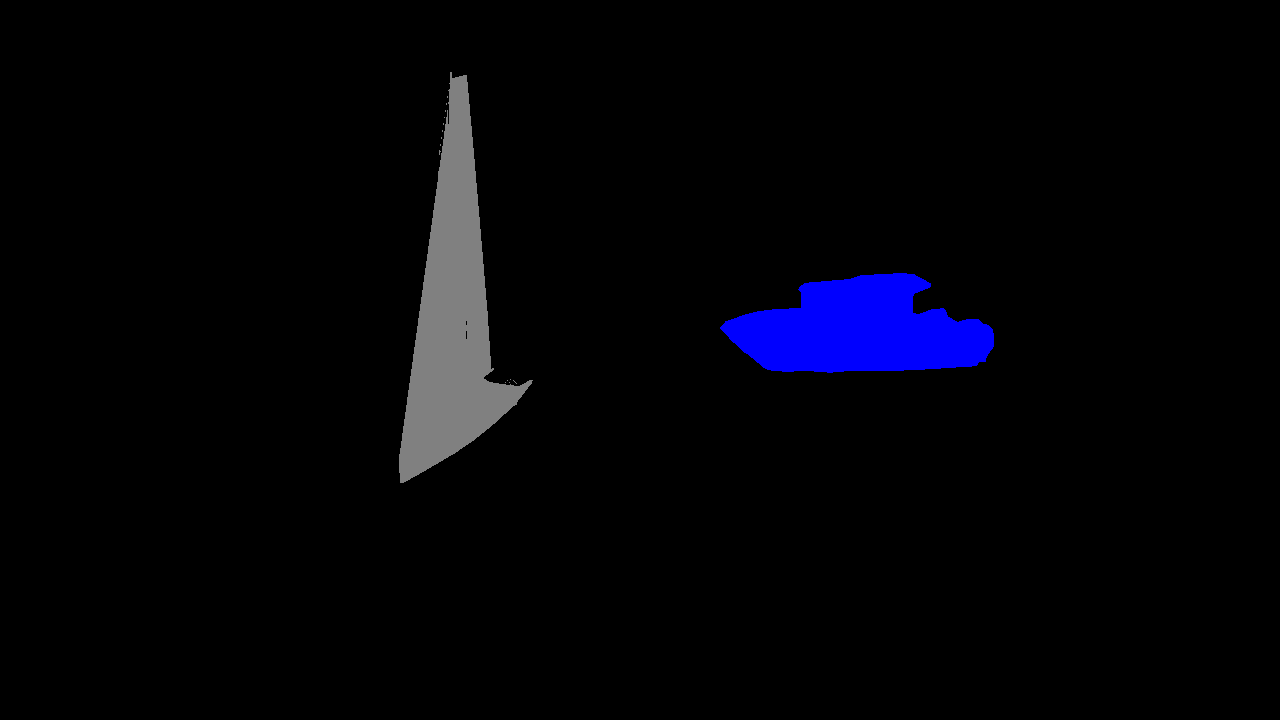
\includegraphics[width=0.7\textwidth]{Figures/segmentation_2.png}
    \caption{Visualization of segmentation, which divide the image into precise pixel-level regions.}
    \label{fig:image3}
\end{figure}



\subsection{Advantages with Synthetic Labeling}
Labeling in synthetic images is a big advantage compare to real images. Using real images requires manual effort for labeling, which involves identifying and annotating each object in the dataset. As dataset sizes grows, manual labeling becomes impractical. Annotating thousands of real-world images needs a lot of human labor and can include inconsistencies, potentially impacting the model accuracy \cite{nikolenko2021synthetic}.\\

\noindent In contrast, synthetic images provide the advantage of automatic labeling during the generation process. Platforms like Unity offer automated labeling capabilities via the Perception Package \cite{unity-perception2022}. This ensures pixel-perfect annotations, including bounding boxes and segmentation masks with no manual intervention. The automated process delivers consistent, high-quality annotations for every image while saving time and effort.


\section{Balancing Realism in Synthetic Data}
While synthetic image generation offers numerous benefits for computer vision models, a key challenge is achieving sufficient realism. The domain gap between synthetic and real-world data can significantly impact model performance \cite{nikolenko2021synthetic}.  Although it is possible to create highly realistic scenes, some aspects remain particularly difficult to simulate. For instance, dynamic surfaces like water in maritime applications can be a challenge due to its complex behavior with reflections and refractions \cite{waterrendering}. Similarly, obtaining realistic 3D renderings of objects like boats and other maritime structures can be difficult.\\

\noindent Going for a realistic synthetic datasets can be expensive and time consuming and may outweigh the benefits. Instead, specific optimizations and techniques can help bridge the gap between synthetic and real-world data \cite{nikolenko2021synthetic, jimaging8110310}. By balancing realism and practicality, synthetic datasets can achieve a level that meets the needs of specific applications without excessive computational costs.


\section{The Future of Synthetic Images}
\label{gan}
Using AI to generate images for computer vision models has become an increasingly powerful tool, with Generative Adversarial Networks (GANs) being popular in this field. GANs consist of two neural networks that work in a competitive process to create realistic synthetic data. The generator produces fake data, while the discriminator evaluates whether the data is real or fake, with both networks improving through this competition. This dynamic has made GANs highly effective for tasks like image generation, domain adaptation and creating privacy-preserving synthetic datasets. Despite their potential, training GANs can be challenging due to the risk of producing data with limited diversity. These challenges can limit the models ability to generalize and innovate \cite{gan}. GANs and other AI-driven innovations are helping reduce the time and cost of creating datasets, while also enabling the simulation of complex scenarios and environments. However, using AI to train AI introduces additional risks such as overfitting and hallucination. This is when models generate outputs that are not only inaccurate but may also be entirely fictional or irrelevant \cite{hallucination}. Hallucinations often arise from poor-quality training data that the model may overfit during training, leading to bad results. Tackling this challenge requires the development of new techniques to detect and correct these errors, ensuring more reliable synthetic data.

\cleardoublepage

\chapter{Theory: Unity}
%equations, bib. \\
Unity is a popular 3D rendering platform widely used for synthetic image generation in computer vision projects. It offers powerful tools, including the Perception package \cite{unity-perception2022}, which simplifies tasks like randomizing object positions and generating labeled datasets. Unity's integration with simulation tools and its large Asset Store \cite{UnityAssetStore} make it an efficient platform for quickly setting up and customizing virtual environments for training machine learning models.

\section{Unity as the Platform Choice}
There are several different 3D rendering platforms such as Blender, Unity and Unreal Engine. Unity was the natural choice for this project for several reasons. Firstly, Unity offers an perception package \cite{unity-perception2022} with a lot of documentation and customization options. It also provide tools for generating labeled datasets, camera simulations and randomization of object positions. Secondly, the DNV simulator used to simulate Revolt boat operates on Unity \cite{dnv_wiki}. By using Unity to generate images, one becomes familiar with the platform, eliminating the need to learn a new platform when working with the simulator. Finally, Unity also has a large asset library called the \textit{Unity Asset Store} \cite{UnityAssetStore}, which includes prebuilt environments, animations and 3D objects. This makes it easy to quickly set up and customize a virtual environment, saving time and effort in the development process. These factors contributed to Unity being the platform of choice for image generation in this project.


\section{Unity Perception package}
The Perception package is a powerful tool that was important for selecting Unity as the 3D platform for this project. The primary purpose of the package is to simplify the process of synthetic image generation \cite{borkman2021unityperceptiongeneratesynthetic}. It includes a range of pre-built randomization algorithms that help create varied and diverse datasets. Additionally, the package also helps with labeling by automatically assigning labels to 3D objects.

\subsection{Object Labeling}
The Unity Perception Package offers an efficient way to produce labeled images. Before generating images, each object must be assigned a labeling component. This allows the Perception Package to generate a segmentation image alongside the original image, enabling the model to accurately learn object locations in each frame.



\subsection{Integrated Randomizers}
\label{section:Integrated Randomizers}
There are several different randomizers included in the Perception package \cite{unity-perception2022}. These are C\# scripts that take in parameters and manipulate objects for each frame. All the randomizers are classes that extend the base class \textit{Randomizer}. The base class provides functions and methods to help building new randomizers. One of the key methods is \texttt{OnIterationStart()}, which runs every time a new iteration or frame is generated for the image. This method is useful for adding logic that changes the scene in different ways on every iteration. The prebuilt randomizers used in this project were the \textit{RotationRandomizer} \cite{rotation_randomizer}, \textit{SunAngleRandomizer} \cite{sun_angle_randomizer} and \textit{ColorRandomizer} \cite{color_randomizer}.

\begin{figure}[H]
    \centering
    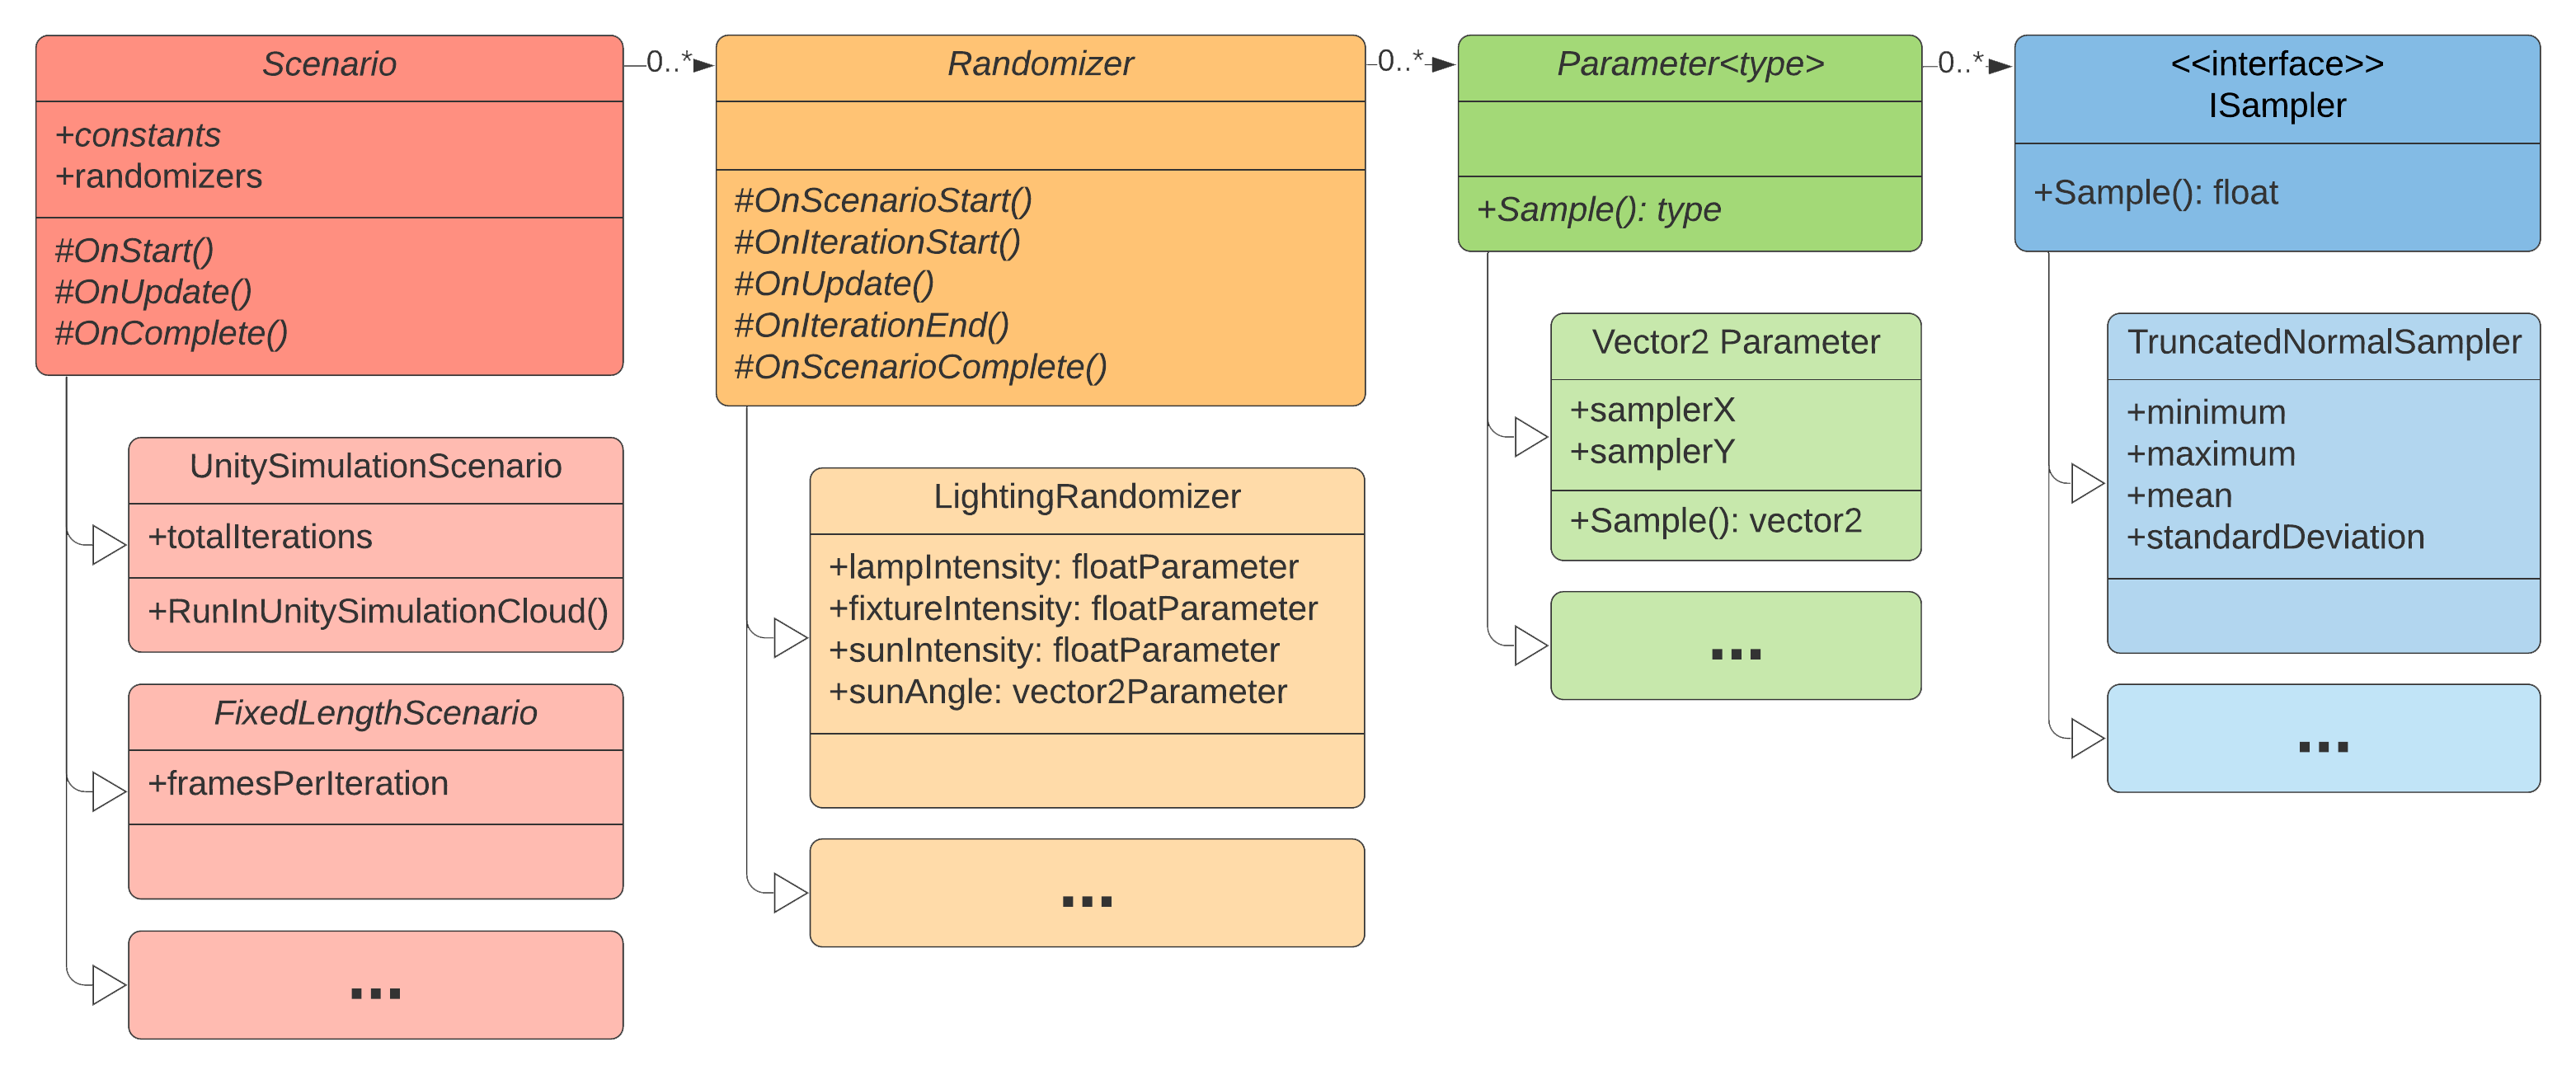
\includegraphics[width=0.99\textwidth]{Figures/randomization_uml.png}
    \caption{UML diagram of the randomization framework in the Unity Perception package, showing the relationships between randomizers, parameters and interfaces. Taken from Unity Perception package documentation \cite{UMLdiagram}.}
    \label{fig:randomizer class uml}
    
\end{figure}

\subsubsection{RotationRandomizer}
The \textit{RotationRandomizer} \cite{rotation_randomizer} applies a random roll, pitch and yaw to a 3D object in each iteration. It builds on the \textit{Randomizer} class and takes in six float parameters: the minimum and maximum rotation for the x, y and z axes. The \texttt{OnIterationStart()} method then runs, which picks a random rotation within the specified ranges. The use of a minimum and maximum is important for this project to ensure the object doesn’t end up upside down or floating in unrealistic positions.

\subsubsection{SunAngleRandomizer}
The second randomizer used is the \textit{SunAngleRandomizer} \cite{sun_angle_randomizer}. This randomizer manipulates the light source connected to the camera to simulate different times of the day. It takes in five parameters: the minimum and maximum for the time of day and the day of the year (where 0 corresponds to January 1st and 356 corresponds to December 31st). The last parameter is the latitude, which is important for calculating the suns position at a given time.

\subsubsection{ColorRandomizer}
The last randomizer used in this project is the \textit{ColorRandomizer} \cite{color_randomizer}. This randomizer allows the randomization of an object's color by adjusting the RGBA (Red, Green, Blue and Alpha) components within specified ranges. It takes parameters for the minimum and maximum values for each of the components, which generates a color variation to objects. Similar to the other randomizers, the \textit{ColorRandomizer} uses the \texttt{OnIterationStart()} method to apply the randomization on each frame.


\subsection{Customizable Randomizers}
Additional randomizers was coded to make the dataset more varied and random than what the perception package offers by default. These custom randomizers control camera positioning, object placement, and environmental effects. All new scripts are written in C\# and are based on the perception class Randomizer.

\subsubsection{Camera Randomizer}
The \textit{Camera Randomizer} generates a new camera position for each frame while ensuring that the camera remains focused on the target object. By extending the \textit{Randomizer} class, this custom randomizer provides control over the camera's distance from the object, as well as its pitch (elevation) and yaw (horizontal rotation) angles. \\

\noindent Spherical coordinates were used to calculate new camera positions. The randomizer takes user-defined ranges for distance, pitch and yaw, and calculates a random value within these ranges for each iteration. These parameters are then converted to Cartesian coordinates using the following equations:

\begin{align}
X_{\text{offset}} &= d \cdot \sin(\phi) \cdot \cos(\theta) \\
Y_{\text{offset}} &= d \cdot \sin(\theta) \\
Z_{\text{offset}} &= d \cdot \cos(\phi) \cdot \cos(\theta)
\end{align}

\noindent In the equations \(d\) is the camera's distance from the object, \(\phi\) is the yaw angle (in radians), and \(\theta\) is the pitch angle (in radians). The equations used to convert spherical coordinates to Cartesian coordinates are based on standard mathematical principles \cite{wolfram_spherical_coordinates}.\\

\noindent The calculated offsets determine the new camera position relative to its initial position. The camera is then rotated to face the target object using Unity's \texttt{Quaternion.LookRotation} function to calculate the rotation. This function takes in \texttt{target.position - offset.position}, which gives the relative position of the target from the camera's current position, and calculates the transformation \cite{unity_quaternion_lookrotation}. This randomizer generates varied camera perspectives, capturing different views of the object, the water-level and background elements.

\begin{figure}[H]
    \centering
    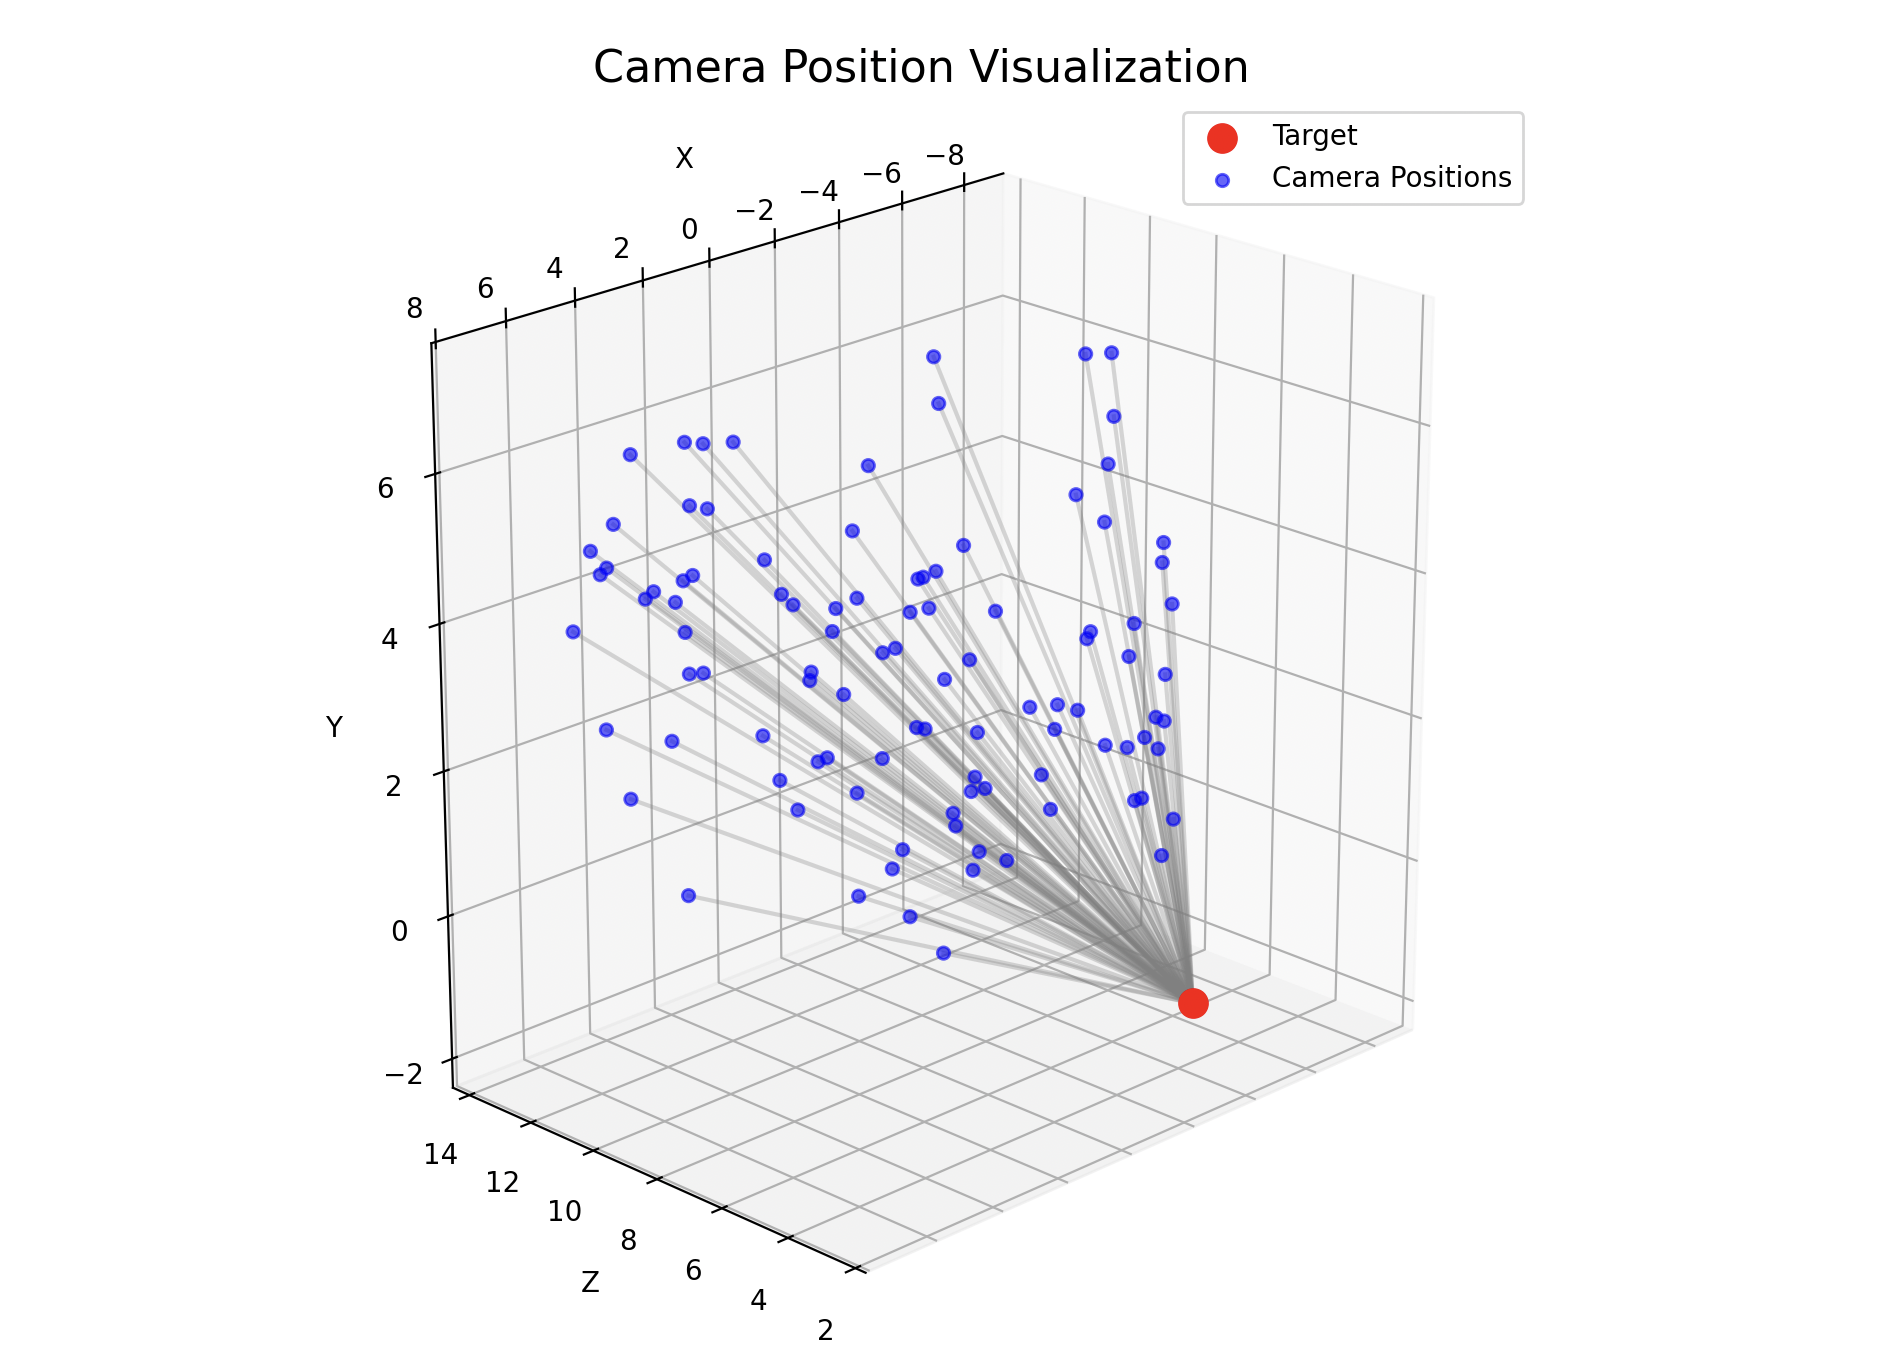
\includegraphics[width=0.7\textwidth]{Figures/camerapos.png}
    \caption{Visualization of new camera positions generated relative to the initial position.}
    \label{fig:camera_randomizer_plot}
    
\end{figure}

\subsubsection{Position Randomizer}
The \textit{Position Randomizer} changes the location of objects within a specified 3D space. It builds on the Randomizer class and allows users to define ranges for the X and Z positions. Random values within these ranges are generated, and the object is moved to a new position while keeping its original Y position unchanged. This ensures the object's height stays the same, as the scene simulate floating objects. This randomizer ensures objects are placed off-center, adding spatial variety.

\subsubsection{Rain Randomizer}
The \textit{Rain Randomizer} enhances the dataset by simulating rain effects during data collection. It includes a parameter that sets how many iterations the rain effect will be applied. After reaching this limit, the rain effect turns off, and the remaining iterations are generated without it. This adds realistic noise and variety to the scene, improving the diversity of the dataset.


\cleardoublepage


\chapter{Method}

In this chapter, the method for generating synthetic images using Unity, a 3D development platform, is outlined. The process begins with the creation of a virtual environment that simulates realistic maritime conditions, incorporating various elements such as water dynamics and weather conditions. Unity's rendering capabilities can generate a diverse set of images that serve as training data for computer vision models. By adjusting parameters such as lighting, camera angles, and object placements, the dataset can that reflects real world scenarios. 


\section{Creating the Virtual Environment}
Creating an virtual environment in Unity involves designing a scene that simulates real-world conditions. A scene in unity consist of two main components: a camera to capture the scene, and a 3D grid to define the spatial layout. Various objects and elements can be added to the 3D space, such as terrain, water, maritime objects and other 3d models. Additionally, animations can be added to simulate dynamic conditions such as water movement or rain which is important to create a realistic environment. 
 
\subsection{Terrain}
Generating terrain in 3D space is a natural starting point for the virtual environment. The Unity \textit{standard asset packages} was used, providing a flat surface as a foundation. This package includes an environmental editor that allows users to manipulate the terrain, adjusting its shape by adding hills and valleys. Additionally, the editor offers options to change the ground type, such as switching from grass to rocks.

\subsection{Water}
The water surface was also imported from Unity's \textit{Standard Asset Packages}, which offers a realistic water simulation. This asset provides a flexible water surface that users can adjust in both position and dimensions to fit the scene. The water is animated with small ripples, ensuring it appears dynamic rather than as a still blue surface. However, the \textit{Standard Asset Package} does not support advanced water conditions, such as large waves. Since this simulation focuses on object detection within a harbor environment, where sea conditions are generally calm, this limitation is not a significant issue.

\subsection{Weather}
To create a realistic environment, there is also important to generate a weather system. \textit{Rain Maker - 2D and 3D Rain Particle System for Unity} was downloaded from Unity asset store and imported the prefab into Unity. This weather system allows for adjustments to rain and fog intensity. Additionally, the rain particles are animated to avoiding repetitive or identical images.

\section{Integrating 3D Models}
After creating the scene and environment, the next step is to integrate the 3D objects that will appear in the generated images. Since the focus is on harbor docking, so the 3D models should represent common objects found in such environments. Common items include motorboats, sailboats, kayaks, buoys, windsurfers, and other small watercraft. The process involves planning to select the right objects, sourcing the models from various platforms, and integrating them into the scene.

\subsection{Sourcing 3D Models}
Several platforms offer free and paid 3D models. Free options were more limited in variety and quality, but they were enough to build a scene. Unity supports various file formats for importing 3D models, including 3DS, FBX, DAE, DXF, and OBJ, which made it easier to work with assets from multiple sources. The primary platforms used to find models were:
\begin{itemize}
\item \textbf{Unity Asset Store}: A platform with many free and affordable assets, and is also integrated with Unity platform. \cite{UnityAssetStore}
\item \textbf{CGTrader}: A marketplace that offers a wide selection of high-quality free 3D models.\cite{cgtrader}
\item \textbf{Sketchfab}: A community-driven platform for uploading, sharing, and discovering 3D models. \cite{sketchfab}
\item \textbf{DNV}: Internal resources from DNV Wiki on DevAzure were also utilized. While it included some usable models suitable for harbor environments, some where large cargo ships, military frigates, and RMS Queen Elizabeth which is not directly relevant.\cite{dnv_wiki}

\end{itemize}

\subsection{Adding 3D Models to the Environment}
Once the models were downloaded, they could be added to the Unity scene. The models were added to the project's asset folder and then could be dragged into the scene in the Unity window. Firstly, a background was added with some buildings and a dock, creating a harbor environment. Then, the different 3D objects were placed in front of the camera. The models where then positioned to be fully visible within the frame. The process involved trial and error to ensure that the scene looked natural and objects where visible in the frame.


\section{Implementation of Randomizers in Unity}
After constructing the environment and importing all objects to be rendered, randomizers were implemented using the Unity Perception Package \cite{unity-perception2022}. Following Unity's perception guide \cite{unity-perception2022} and the YouTube tutorial \textit{Creating Randomized Synthetic Images with Unity3d Perception} \cite{secrets_of_apagayo_island_video}, the process involved the following steps:

\begin{itemize} \item \textbf{Create a Scenario}
The scenario object manages the randomization process and specifies the number of images to generate. It connects the randomizers to the environment, ensuring they work together to create a varied dataset. The scenario runs when the scene is played and coordinates all randomizers in a defined order.\cite{borkman2021unityperceptiongeneratesynthetic} The scenario can easily be added by dragging it from the perception package into the scene. For this project, the scenario was configured to generate 100 images, with parameters such as the number of frames and intervals set in Unity’s interface.

\item \textbf{Create Custom Randomizers}: 


\item \textbf{Add Randomizers to the Scenario}: Randomizers introduce changes to specific aspects of the scene, such as camera positions, object colors, and lighting conditions. Six randomizers were used: camera, sun angle, color, position, transformation, and weather randomizers. Each randomizer was added to the scenario and configured with parameters to control the range of variation. Most Parameters required trial and error to ensure a balanced dataset. Randomizers could also be linked to objects like the camera, so it could interact with those elements during the randomization process.

\item \textbf{Apply Randomization Tags to 3D Objects}: When randomizers are added to a scenario, most are not connected to the objects. Different randomizers can be applied to various elements, such as foreground and background objects, and some may affect multiple objects. To specify which objects to manipulate, add a \texttt{randomization tag} component to each object. This tag directs the randomizer script to apply transformations to the tagged object.

\item \textbf{Label Objects for Ground Truth Data}: Labeling objects is essential for obtaining ground truth data. To do this, add a \texttt{Labeling} component to each object and assign it a name. This component, which is a script included with the package, enables labeling functionality. Next, go to the camera object and add the label name to both the BoundingBox and Semantic- SegmentationLabeler. This ensures that Unity generates an RGB image for each frame along with a corresponding segmentation image.

\item \textbf{Generate Images}: Once setup is complete, play the scene to start the randomization process. Unity generates synthetic images with defined randomizers and parameters, creating a diverse dataset.
\end{itemize}


\section{Use of Ai-tools}
\subsection{Literature study}
\subsection{Coding}
\subsection{Writing}

% \section{generating ir images}


\cleardoublepage


\chapter{Results}
The primary result of this project is a synthetic image dataset generated using Unity, offering an alternative to real-world images for training and testing machine learning models. The dataset consists of 2350 images with various boats and maritime objects in a harbor environment. It showcases the capabilities of the Unity Perception package, including the use of diverse scenarios with varying camera positions, weather effects and object orientations. These features increase the dataset's diversity for machine learning tasks, helping to create better models. A link to the GitHub repository containing the dataset and additional resources can be found in Appendix A.

\section{Dataset}
The dataset contains synthetic images of objects in a harbor environment, created entirely using Unity. Objects in the dataset include boats, sailboats, kayaks and buoys, with variations in environmental conditions such as rain.\\

\noindent The distribution of object types and their corresponding weather conditions is summarized in Table~\ref{tab:dataset_composition}. Each object type has been rendered under various conditions to ensure a realistic and comprehensive dataset for training machine learning algorithms.
 
\begin{table}[H]
\centering
\begin{tabular}{|l|c|}
\hline
\multicolumn{2}{|c|}{\textbf{Dataset Distribution}} \\ 
\hline
\textbf{Object Type} & \textbf{Total Appearances}\\ 
\hline
Boats         & 2100  \\ 
Small rib     & 200 \\
Sailboat      & 900     \\
Sailboat without sail     & 800    \\
Kayak        & 1100     \\ 
Buoy         & 200     \\ 

\hline
\textbf{Total}       & \textbf{5300} \\ 
\hline
\end{tabular}
\caption{Breakdown of the dataset by object type.}
\label{tab:dataset_composition}
\end{table}



\begin{figure}[H]
\centering
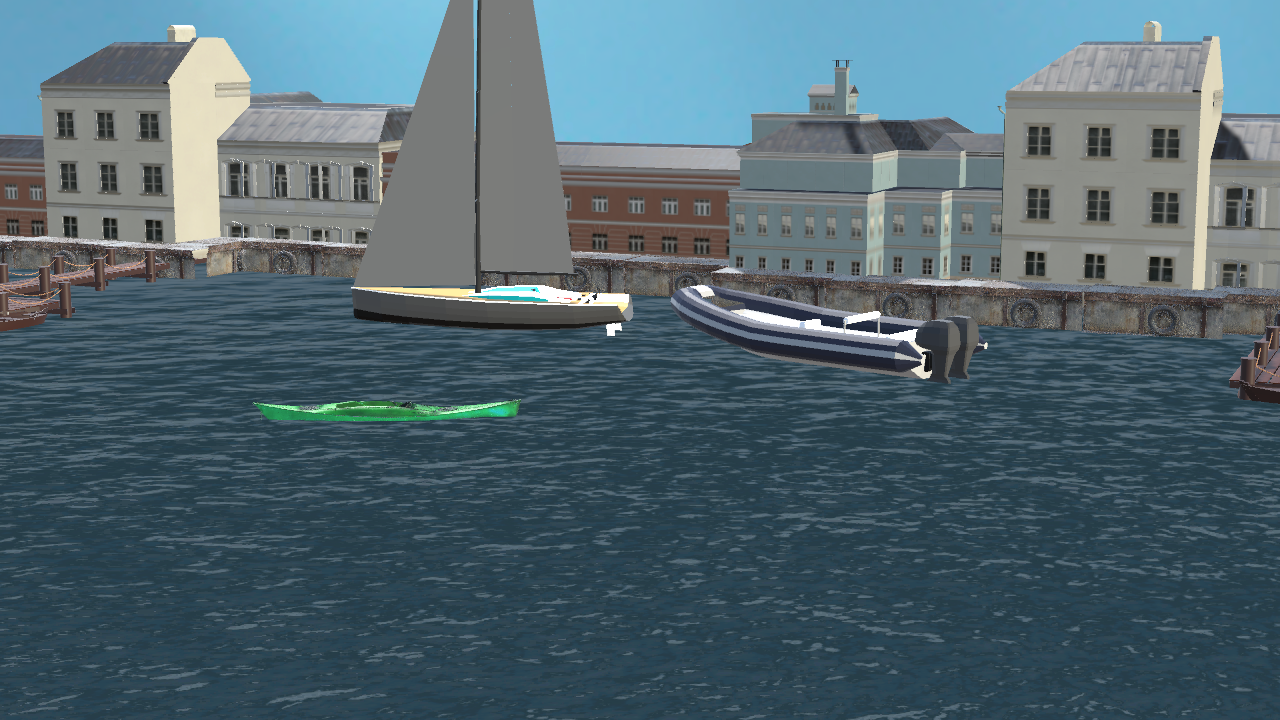
\includegraphics[width=0.8\textwidth]{Figures/results/rand2.png}
\caption{Example of one of the images in the dataset.}
\label{fig:original_image}
\end{figure}

\section{Dataset Diversity}
A key goal of this project was to create a dataset that captures a wide range of scenarios. The results demonstrate a highly varied dataset with changes in object rotations, positions and weather conditions. Ensuring diversity in the dataset helps make it more generalizable, improving model performance in different situations. However, one aspect that could be further improved is the variety of backgrounds, which is quite similar in all the images. \\

\noindent Figure \ref{fig:randomized_images} shows examples of randomized images with the same target object. These examples highlight how randomization creates variety in rotation, background and camera position.

\begin{figure}[H]
\centering
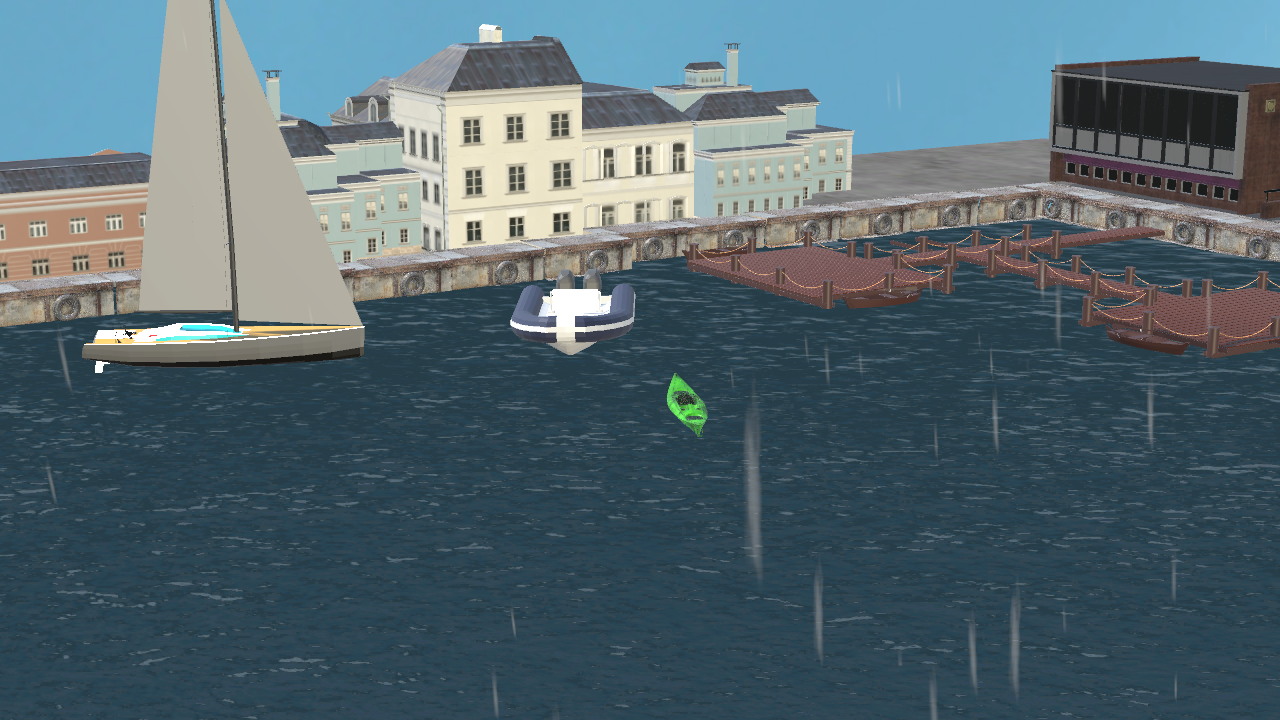
\includegraphics[width=0.32\textwidth]{Figures/results/rand1.png}
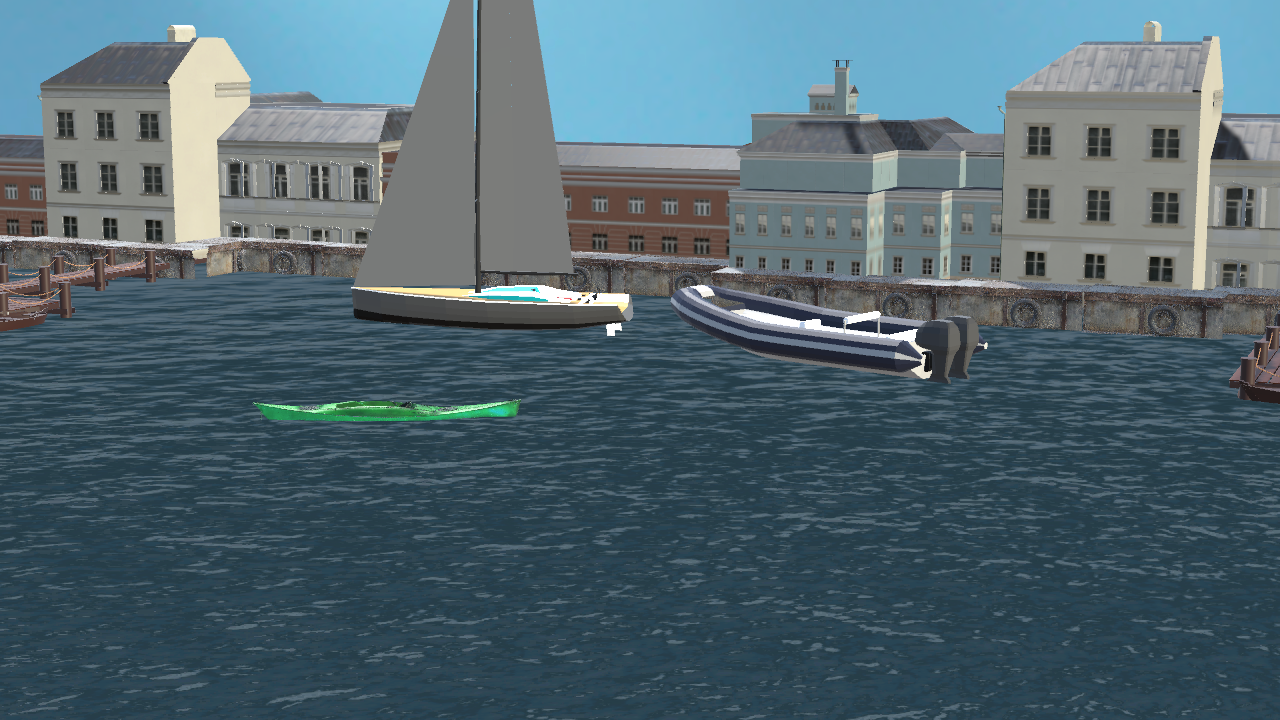
\includegraphics[width=0.32\textwidth]{Figures/results/rand2.png}
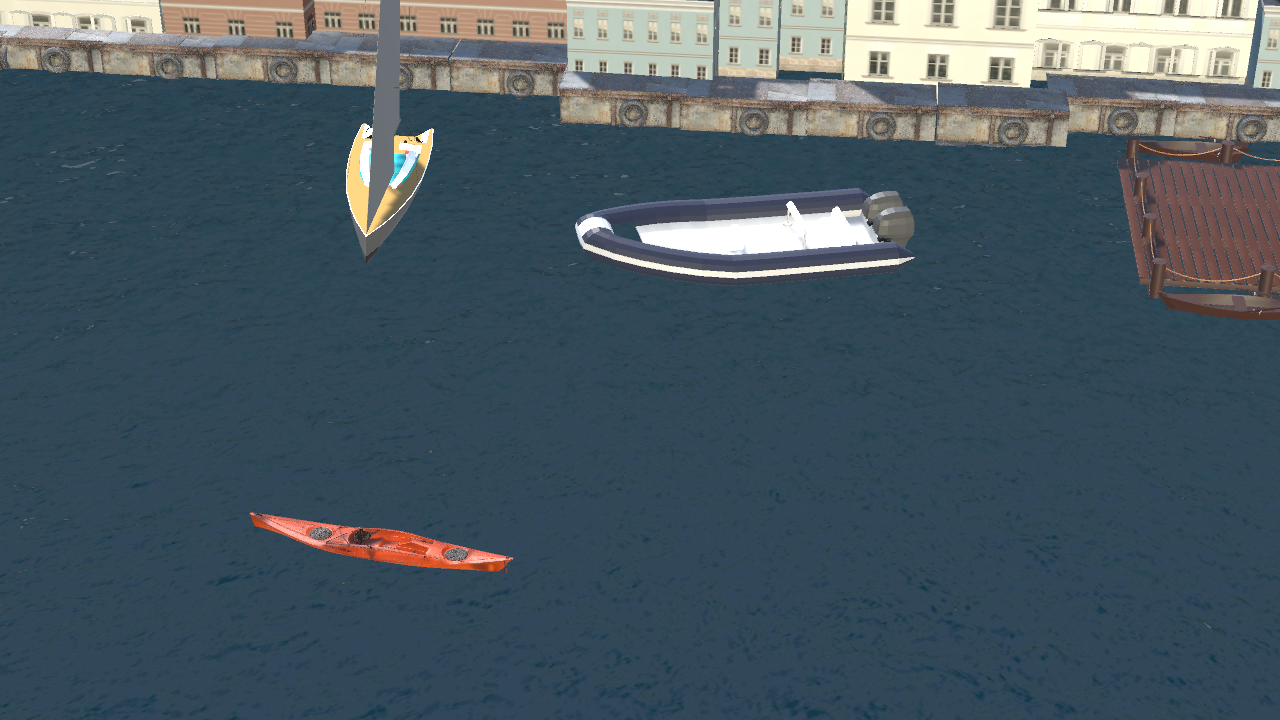
\includegraphics[width=0.32\textwidth]{Figures/results/rand3.png}
\caption{Example of 3 randomized images with the same target.}
\label{fig:randomized_images}
\end{figure}

\section{Labeling}
Labeling is important because it helps computer vision models identify and learn the objects in an image \cite{Labelling}.  The results from the generation included two images for each scene: the original image and a corresponding segmentation image, where each object is marked with a distinct color. This dual-image output provides a clear connection between the visual data and the labels, ensuring consistency in training.\\

\noindent Figure \ref{fig:labeled_images} shows an example of the labeling process. The left image is the original and the right image is the segmented version. This comparison shows how well the labels match the objects in the original image, ensuring the model learns from accurate data.

\begin{figure}[H]
\centering
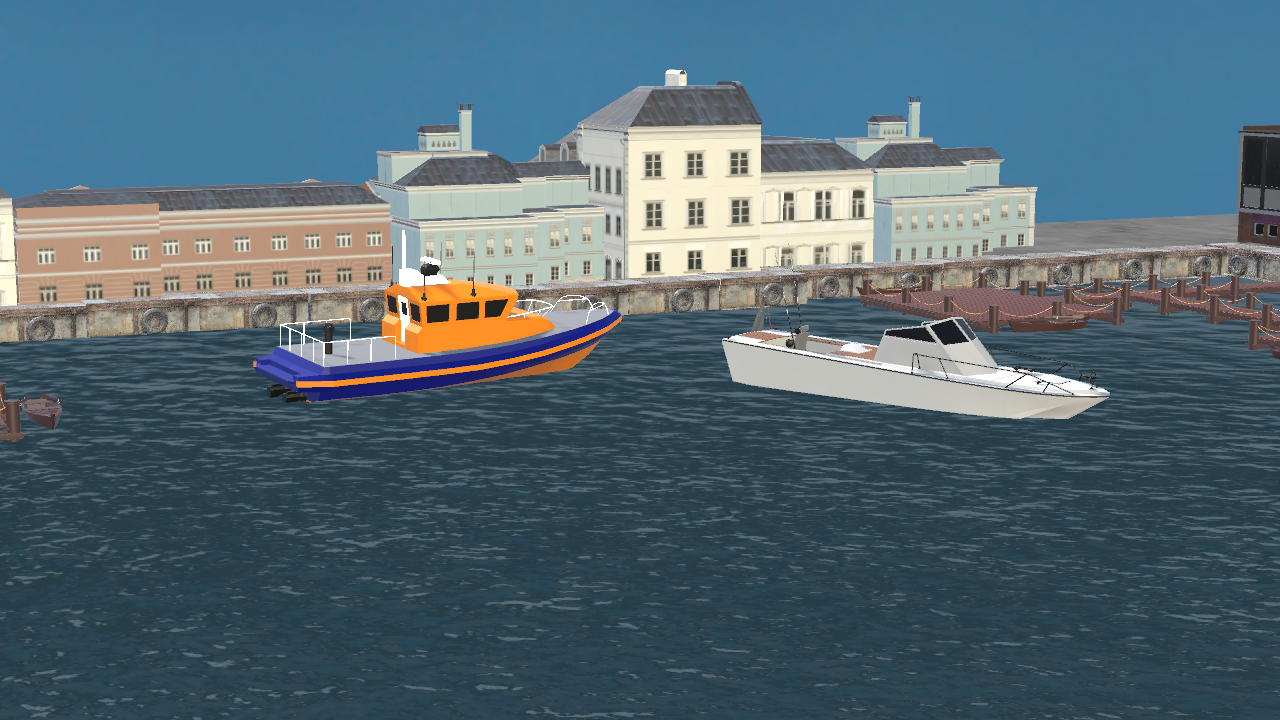
\includegraphics[width=0.49\textwidth]{Figures/results/rgb_105.png}
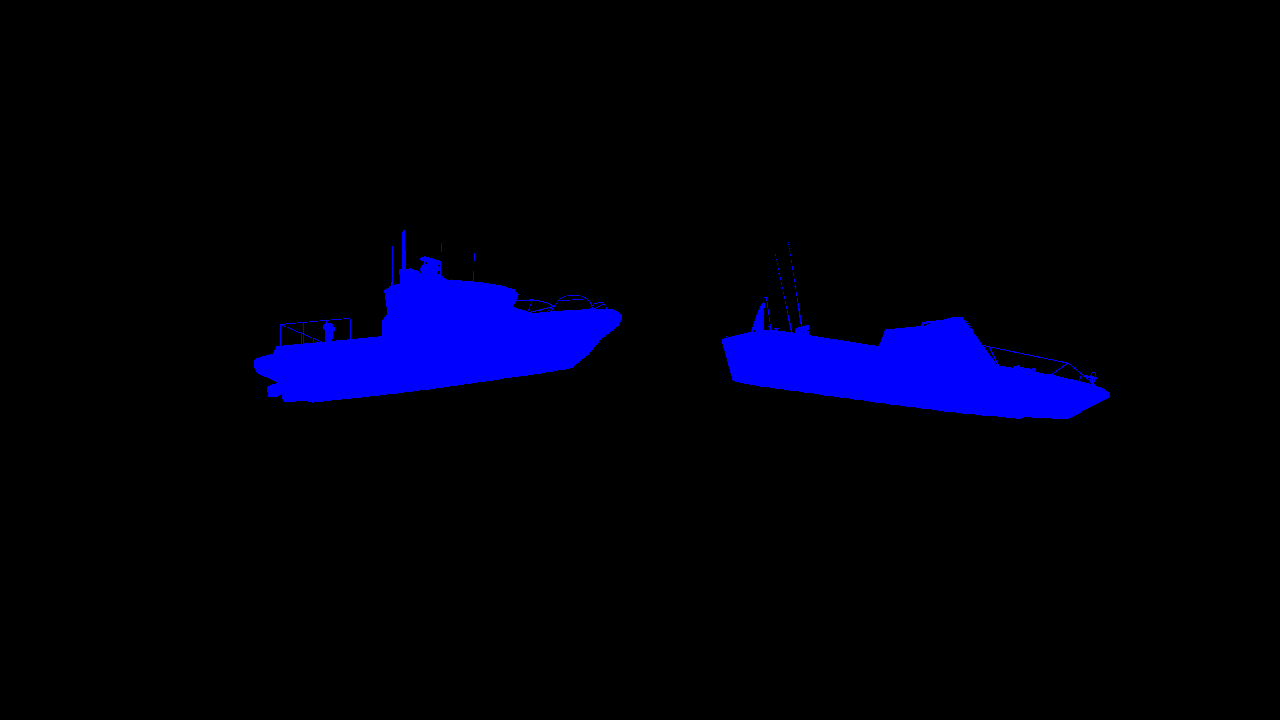
\includegraphics[width=0.49\textwidth]{Figures/results/segmentation_105.png}
\caption{Comparison of the original image and its labeled segmentation output.}
\label{fig:labeled_images}
\end{figure}


\cleardoublepage





\chapter{Conclusions}

This project has shown promising results, demonstrating Unity's potential as a platform for synthetic data generation. Unity proved to be an effective platform for generating synthetic data, thanks to its Perception package, which streamlined image generation, randomization and labeling. The resulting dataset comprises diverse and well-labeled images that can serve as a foundation for computer vision model training.\\

\noindent The experience with Unity highlighted its advantages, such as the ease of integrating 3D models and its flexibility in creating realistic and diverse datasets. However, the effectiveness of the dataset in training robust computer vision models cannot be fully assessed until model training is completed.


\section{What Has Been Done}
The main accomplishments of this project include: 
\begin{itemize} 
\item Creating a virtual environment in Unity for simulating a harbor docking scenario. 
\item Integrating 3D models representing common maritime objects such as boats, buoys and docks. 
\item Generating a synthetic dataset using the Unity Perception package, incorporating features such as randomized object placement, lighting and weather conditions. 
\item Producing labeled data, such as segmentation masks to help training of computer vision models. 
\item Exploring the use of AI tools to enhance the realism of the dataset. 
\end{itemize}
  
\noindent This establish a solid groundwork for exploring the potential of synthetic data in computer vision applications.

\section{Future Work}
Future work will focus on addressing the research question: Is synthetic data sufficient to train a computer vision model for harbor environments, or is real-world data necessary to achieve acceptable performance?\\

\noindent This will involve training various models with the synthetic dataset, collecting real-world data and testing the model's ability to generalize. It is also interesting to evaluate the impact of combining synthetic and real-world data versus using synthetic data alone.\\

\noindent This work will continue in the spring as part of my master's thesis and is set to be an exciting and challenging next step.

\cleardoublepage


\addcontentsline{toc}{chapter}{\protect\numberline{}References}
\printbibliography[title={References}] %you may change the title in the toc here if you want
\cleardoublepage


\chapter*{\LARGE \textbf{Appendices}}
\fancyhf{} %clear the header, it should be empty for the appendices
\renewcommand{\headrulewidth}{0pt} %no rule
\fancyfoot[C]{\thepage} %set the page numbers in the center of the footer instead 

%it is possible to set a different page numbering style for the appendix, but I personally just continued with the same page numbering as the main content as I find that more tidy
%\pagenumbering{roman}
%\setcounter{page}{1}
\addcontentsline{toc}{chapter}{\protect\numberline{}Appendices:}
\appendix
\chapter*{A - Github repositories}
\addcontentsline{toc}{chapter}{\protect\numberline{}A - Github repositories} 


\subsection*{Latex repository link}
\begin{itemize}
    \item \url{https://github.com/trygvemm/Project_Thesis_Latex.git}
\end{itemize}
\subsection*{Unity repository link}
\begin{itemize}
    \item \url{https://github.com/trygvemm/UnitySyntenticImages.git}
\end{itemize}
\subsection*{Dataset repository link}
\begin{itemize}
    \item \url{https://github.com/trygvemm/Unity_dataset.git}
\end{itemize}





\chapter*{B - Assets Download Links}
\addcontentsline{toc}{chapter}{\protect\numberline{}B - Assets Download Links} 

%For included tables and figures renew the numbering such that they are numbered by the appendix they are attached to and not to the conclusion chapter
\renewcommand{\thefigure}{B.\arabic{figure}}
\setcounter{figure}{0}
\renewcommand{\thetable}{B.\arabic{table}}
\setcounter{table}{0}


\section*{\large{B1 - Table of Download Links}}
\vspace*{1cm}

\begin{table}[H]
\centering
\begin{tabularx}{\textwidth}{|l|X|}
\hline
\textbf{Object Name} & \textbf{Download Link} \\ 
\hline
Bouy            & \href{https://www.cgtrader.com/items/3704851/download-page}{https://www.cgtrader.com/items/3704851/download-page} \\ 
Boats               & \href{https://www.cgtrader.com/3d-model/boats-db796996-1477-4b6e-848a-11a92d688845}{https://www.cgtrader.com/3d-model/boats-db796996-1477-4b6e-848a-11a92d688845} \\ 
Dock                & \href{https://sketchfab.com/3d-models/rusty-dock-c962b46f71e144fc9fb397a251dfeee9\#download}{https://sketchfab.com/3d-models/rusty-dock-c962b46f71e144fc9fb397a251dfeee9\#download} \\ 
Kayak               & \href{https://sketchfab.com/3d-models/kayak-summer-fun-6d77716d39024d49b4c8840a8d2ca53b\#download}{https://sketchfab.com/3d-models/kayak-summer-fun-6d77716d39024d49b4c8840a8d2ca53b\#download} \\ 
House           & \href{https://assetstore.unity.com/packages/3d/props/exterior/urban-building-130318}{https://assetstore.unity.com/packages/3d/props/
exterior/urban-building-130318} \\ 
Rain            & \href{https://assetstore.unity.com/packages/vfx/particles/environment/rain-maker-2d-and-3d-rain-particle-system-for-unity-34938}{https://assetstore.unity.com/packages/vfx/particles/environm
ent/rain-maker-2d-and-3d-rain-particle-system-for-unity-34938} \\ 
Houses          & \href{https://assetstore.unity.com/packages/3d/environments/urban/town-houses-pack-42717}{https://assetstore.unity.com/packages/3d/environments/urb
an/town-houses-pack-42717} \\ 
Skybox          & \href{https://assetstore.unity.com/packages/2d/textures-materials/sky/fantasy-skybox-free-18353}{https://assetstore.unity.com/packages/2d/textures-materials/sky/fantasy-skybox-free-18353} \\ 
\hline
\end{tabularx}
\caption{Download links for all 3D assets.}
\label{tab:download_links}
\end{table}



\end{document}
